\documentclass[twoside,12pt,a4paper]{article}

\newcommand{\bhamstudentname}{Ziyan Wang}
\newcommand{\bhamthesistitle}{Secure E2EE Chat System}
\newcommand{\bhamfronttitle}{Secure E2EE Chat System\\Based on Signal Protocol}
\newcommand{\bhamschool}{School of Computer Science}
\newcommand{\bhamcollege}{Engineering and Physical Sciences}
\newcommand{\bhamdegree}{MSc. Computer Science}
\newcommand{\bhamid}{2014988}
\newcommand{\bhamsupervisor}{Dr Mihai Ordean}
\newcommand{\bhamyear}{2020}

\usepackage{enumerate}
\usepackage[hyphens]{url}
\usepackage[breaklinks]{hyperref}
\usepackage{fancyhdr}
\usepackage[sort]{natbib} 
\usepackage{comment} % from http://www.latex-community.org/forum/viewtopic.php?f=5&t=4538
\usepackage{dirtree} % from http://blog.plenz.com/2011-07/represent-directory-structures-in-latex.html
\usepackage{longtable} % from http://stackoverflow.com/questions/2896833/how-to-stretch-a-table-over-multiple-pages
\usepackage{algorithm}   
\usepackage{algorithmic}   %both algorithm* from http://hasini-gunasinghe.blogspot.co.uk/2014/02/presenting-algorithmsprotocols-in-neat.html

\renewcommand{\algorithmiccomment}[1]{#1} %http://tex.stackexchange.com/q1uestions/61861/algorithmic-package-for-loop-and-comment-at-the-same-line

\pagestyle{fancy}
\renewcommand{\sectionmark}[1]{\markboth{#1}{}}	%from tex.stackexchange.com/questions/111361

\lfoot{\bhamstudentname}
\cfoot{}
\rfoot{}
\fancyhfoffset[L]{0cm} %this fixes the right page number margin issue.
\newcommand{\HRule}{\rule{\linewidth}{0.5mm}}
\renewcommand{\headrulewidth}{0pt}
\newcommand{\tab}{\hspace*{1.25em}}
\newcommand{\minitab}{\hspace*{0.25em}}

%footnote stuff
\usepackage{perpage}
\MakePerPage{footnote} %the perpage package command
\renewcommand*{\thefootnote}{\fnsymbol{footnote}}

\lhead{}\chead{}\rhead{}
\setlength{\headheight}{28pt} %fixes the warnings about headheight being too small
\setlength{\headsep}{6pt}
\pdfoutput=1 % we are running PDFLaTeX
\usepackage[left=2.55cm,right=1.6cm,top=1.8cm,bottom=1.8cm]{geometry}
\usepackage{titling}	
\setlength{\droptitle}{-2.75cm}   % This is your set screw\\
\usepackage{titlesec}
\titleformat*{\section}{\normalsize	\bfseries}
\titleformat*{\subsection}{\small \bfseries}
\titleformat*{\subsubsection}{\footnotesize \bfseries}
%modifies the size of the gaps between the top of the title and bottom
% arguments {type}{left}{top}{bottom}
\titlespacing*{\section} {0pt}{3ex plus 1ex minus .2ex}{2ex plus .2ex}
\titlespacing*{\subsection} {0pt}{2.25ex plus 1ex minus .2ex}{0.75ex plus .2ex}
\titlespacing*{\subsubsection}{0pt}{2.ex plus 1ex minus .2ex}{0.5ex plus .2ex}

\setlength{\intextsep}{0pt} %from http://tex.stackexchange.com/questions/25828/how-to-remove-change-the-vertical-spacing-before-and-after-an-algorithm-environ

\usepackage[pdftex]{graphicx}
\usepackage{enumitem}
\usepackage{pdfpages}
\usepackage{lastpage}
\usepackage{amsmath}
\usepackage{amsfonts}
\usepackage{amssymb}


\usepackage{epstopdf} %http://dirkraffel.com/2007/11/19/include-eps-files-in-latex/comment-page-2/

\usepackage{listings}
\lstset{
 basicstyle=\ttfamily,
  columns=fullflexible,
  keepspaces=true,
breaklines=true
} %from http://tex.stackexchange.com/questions/121601/automatically-wrap-the-text-in-verbatim

\newcommand{\todo}[1]{\textcolor{red}{TODO: #1}\PackageWarning{TODO:}{TODO found: #1!}} %from http://tex.stackexchange.com/questions/9796/how-to-add-todo-notes

\DeclareGraphicsExtensions{.jpg}
%%%%%%%%%%%%%%%%%%%%%  END of TEMPLATE %%%%%%%%%%%%%%%%%%%%%

\title{MSc. Project\\\bhamthesistitle}
\author{\textsf{\bhamstudentname}}

\date{}

\begin{document}

\pagenumbering{gobble} % fix at	 http://tex.stackexchange.com/questions/7355/how-to-suppress-page-number
% this came from http://en.wikibooks.org/wiki/LaTeX/Title_Creation and http://tex.stackexchange.com/questions/14778/error-with-hrule
\begin{titlepage}
\begin{center}
% this was from http://tex.stackexchange.com/questions/7219/how-to-vertically-center-two-images-next-to-each-other
\begin{minipage}{6in}
  \centering
  \raisebox{-0.5\height}{
\includegraphics[width=1.25in]{./resources/crest}}
  \hspace*{.2in}
  \raisebox{-0.5\height}{
\includegraphics[height=0.9375in]{./resources/uni}}
  \end{minipage}
  \\ [1.0cm]
\textsc{{\LARGE \bhamschool\\}College of \bhamcollege}\\[3.5cm]

\textsc{\Large MSc. Project}\\[0.5cm]

% Title
\HRule \\[0.4cm]
\begin{center}\Huge
\bhamfronttitle
\end{center}
\HRule \\[1.5cm]
% Team and Members

\begin{center}
Submitted in conformity with the requirements\\ for the degree of \bhamdegree\\
\bhamschool\\ University of Birmingham\\
\vspace{2cm}
\bhamstudentname\\
Student ID: \bhamid\\
Supervisor: \bhamsupervisor      
\end{center}
\vfill

% Bottom of the page
{\large September \bhamyear}

\end{center}
\end{titlepage}
%\cleardoublepage
\clearpage
\section*{Declaration}
% Taken from the MSc Thesis template, and edited for a PGT report
The material contained within this report has not previously been
submitted for a degree at the University of Birmingham or any other university.
The research reported within this report has been conducted by the author
unless indicated otherwise.\\


Signed ..........................................................................................................................................
\vfill

\maketitle
\vspace{-5.5em} %fixes distance between \maketitle and the TOC
\begingroup
    \fontsize{9pt}{11pt}\selectfont    
    
\tableofcontents

\endgroup
\clearpage
\phantomsection

\section*{Table of Abbreviations}
\begin{itemize}[nolistsep]
\item E2EE -- End To End Encryption
\item jdk -- Java Development Kit
\item TLS -- Transport Layer Security
\item AES -- Advanced Encryption Standard
\item MVC -- Model View Controller
\item bham -- University Of Birmingham
\item DH -- Diffie-Hellman Algorithm
\item X3DH -- Extended Triple Diffie-Hellman Algorithm
\item KDF -- Key Derivation Function
\item MIMA -- Man In The Middle Attack
\item KV pair -- Key Value Pair
\item SSH -- Secure Shell
\item I/O -- Input/Output
\item jdbc -- Java Database Connectivity
\end{itemize}

\addcontentsline{toc}{section}{Table of Abbreviations} 
\clearpage
% set up the page numbering and counter - Table of Abbreviations has no page number
% also set up the footers and headers appropriately.
\pagenumbering{arabic}
\setcounter{page}{1}
\lhead{}\chead{MSc. Project Report :: \nouppercase{Section \thesection\minitab :: \leftmark}}\rhead{}
\rfoot{Page \thepage \hspace*{0.2pt} of \pageref{LastPage}}
\renewcommand{\headrulewidth}{0.4pt}

\section{Overview}
This paper is about upgrading a chat system using Signal Protocol to implement a secure end-to-end-encryption chat system. This report focus on having a brief introduction about Signal Protocol and describing how to implementing a Signal Protocol based end-to-end-encryption system including on client, server and database sides.

The existing chat system is developed myself previously using gradle6 and jdk11. To improve the security of the communication, the project using Signal Protocol to encrypt the messages including on client, server and database sides.

\subsection{Abstract}
As people’s awareness of safety increases, normal symmetric encryption and asymmetric encryption like TLS, AES cannot satisfy their needs: even though the security of transmission can be guaranteed, the server still needs to decrypt the encrypted messages. So once the malicious people use it to get users' sensitive information on server side, users' privacy will be leaked. Besides, the normal symmetric and asymmetric encryptions keep  using the same cipher key during the transmission, once the hacker cracks one encrypted package, the previous and future encrypted packages will be exposed immediately.

In this situation, the Signal Protocol is developed to solve this problem. It implement an end-to-end-encryption protocol to make sure only the call parties can decrypt the encrypted messages, and the cipher key will be changed in each transmission round which can not be referred forward or backward. The server does not decrypt the messages but only forwards the packages to the right users and the database also does not store the decrypted messages from users which greatly reduce the risk of user privacy leakage.

This report describes the fundamental of Signal Protocol and the whole process of implementing it on a existing chat system including on client, server and database sides. On client side, users' communication messages are encrypted by Signal Protocol, only the receiver and other essential information are exposed to the outside. On server side, the server handle the received packages corresponds to their type and only forward the encrypted messages to the corresponding users. Server does not use the libsignal-protocol-java packages which can guarantee the server cannot decrypt the messages. On database side, it only stores users' public keys for other users initializing the pairwise chat, so once the database is breached, there is no damage caused to users.

At the end, the project implements an end-to-end-encryption chat system including pairwise chat, group chat, local history messages storage, multi-device system and message backup functions etc.

Keywords: Signal Protocol, end-to-end-encryption, chat system

\subsection{Acknowledgements}
The success of the project cannot be separated from the help of many people and papers.

First I need to appreciate my Project Supervisor, Mihai Ordean, we have a detailed meeting every week. After each meeting, I can find new directions and questions. Also it's his progress to let me set this subject which I have never touched before.

I also need to thanks my friends, who have given me a lot of advice about this project and listened to my new ideas and my own explains to the project.

Finally, I need to appreciate my family, they spend endless hours to support my project by helping me find the related papers and test the project's robustness which is significant to the development of the project.

\clearpage
\section{Introduction}
\subsection{Overview}
The aim of the work described in this Report is to improve the security of a chat system based on Signal Protocol which people can be not worried about their privacy leakage.
\subsection{Problem statement}
Under the rapid development of the information age, the encryption protocol also have a new revolution. At the beginning, people transmit the messages in plain text which is a original way and information can be obtained easily. So symmetric encryptions born in this situation. The call parties need to negotiate a common cipher key to encrypt the messages during communication. Although the symmetric encryption is quite difficult to crack. But the benefits of cracking are huge. So maybe the hacker will monitor on several days' packages and spend some times to crack the encrypted messages to get the cipher key. And then the he can decrypt any other messages before or after without the knowledge of both parties. Besides, the common cipher key's exchange is also a problem, call parties need to negotiate it via a safe way such as face to face or the cipher key can be obtained by malicious people.

To solve the symmetric encryption's key exchange problem, asymmetric encryption is developed. The server and client will use some asymmetric algorithms to obtain the future common symmetric cipher key. The progress is the security of transmission is improved, the hacker cannot get the common symmetric cipher key easily while two parties are exchanging it. However, the problem mentioned before is still not solved: once the hacker cracks one of the packages, all the packages are exposed to the hacker which will cause unpredictable losses. Besides, the credit of server is also a problem. Usually the call parties are client and server, server decrypt encrypted messages from clients and then forward them to the corresponding users or store them in database. Which means, some unethical companies may sell users' chat history or the hackers can focus on attacking the database to get the information, both of them can have serious consequences.

In this situation, the public needs a new protocol to protect their privacy. Whisper is a good inspiration to develop a new protocol. Only the two parties of communication know what they are talking about. The server are only responsible for forwarding users' messages but not decrypting them. Also, the server does not store the decrypted even encrypted messages in database to make sure the security of users' privacy is guaranteed by users themselves. That is the original purpose of Signal Protocol. It not only combines the symmetric and asymmetric encryption, but also adds a new algorithm to provide forward and future security: Double Ratchet.

\subsection{Project aim}
This project is aim to implement an E2EE chat system using Signal Protocol which can improve the communication security of it. The project does not only develop an E2EE chat program, it focuses on a whole E2EE chat system including server, client, database sides. 

\subsection{Project structure}
The existing chat system is developed by jdk11 and gradle6. It can be divided into three parts: client, server and database. The client is developed using javafx11, it uses MVC architecture to link the data and view. In transmission aspect, it uses socket programming to communicate with server. The communication package has a specific format: each package has a type, both client and server will handle the package corresponding to each type.

On server side, it connects to the bham's database via bham's SSH service.
The database uses PostgresSQL database which served by bham.

The project's main work is on client side where the Signal Protocol encrypt the chat messages of user. The client implements several functions such as pairwise chat, group chat, chat history storage and history messages backup etc. On server side, most of the work is about how to handle the packages from client. For example, server needs to response to users' key bundle requests and forwards the packages to the right users. In database, it simplify the structure of tables, because there is no need to store the chat data in database. But some creation and modification are needed to achieve a Signal compatible system like create a new table to store users' key bundles, add deviceId field in users table to implement a multi-device system.

\subsection{Outline of each section}
In the next set of sections, the report introduce the further related knowledges and the specific implementation and the final result of the system.

In chapter 3, the report introduce some further background materials that reader needs to know to understand the solution. It focuses on how Signal Protocol works and the context of related existing work.

In chapter 4, the report describes the user specification of system, main design of solution and concrete implementation of upgrading the chat system using Signal Protocol including client, server, database sides. It also shows how the project and the writing of a substantial piece of software is managed. Finally, the report presents the whole implemented system's usage result to discuss its success and robustness.

In chapter 5, the report summarise the achievements and the deficiencies of the project. The things that could or would have done are listed for further evaluation.

In chapter 6, the report give a brief statement of how the solution addresses the problem stated at the beginning and provide an evaluative statement based on the results.

In chapter 7, the report explains the file structure of the code and introduces how to run the project code in detail. The proposal and schedules are also presented in this chapter.

\clearpage
\section{Background}
\subsection{Overview}
This project is about implementing an E2EE chat system using Signal Protocol. So understanding how Signal Protocol works is essential in both development and reading. Only after having a deep understanding of Signal Protocol, the whole work can be processed smoothly.

This project uses the libsignal-protocol-java package to develop the Signal Protocol part. However, the documentation of it is not enough to support the new developer to use it. Reading related papers, user guide of related commercial products and the source code of the lib is quite useful.

In this chapter, the report will have a introduction about how Signal Protocol works and how it's implemented in related existing commercial products.

In section 3.2.1, the report presents the Double Ratchet algorithm and gives an introduction of how it works. Section 3.2.2 presents how X3DH algorithm works in Signal Protocol. This two algorithms constitute the core of the Signal Protocol. Finally, section 3.2.3 shows how the whole Signal Protocol works by using this two algorithm.

\subsection{Signal Protocol}
The Signal Protocol is designed by Moxie Marlinspike and Trevor Perrin from Open Whisper Systems. Open Whisper Systems wanted to develop
a new end-to-end encryption standard which works in both synchronous and asynchronous messaging environments. The goals of Signal include end-to-end encryption and advanced security properties such as forward secrecy and future secrecy.

The core parts of Signal Protocol can be divided into Double Ratchet algorithm and X3DH algorithm. This two guarantee the essential features of Signal Protocol such as forward security, future security and asynchronous.

\subsubsection{Double Ratchet}
The Signal Protocol is designed to solve one of problems that once the hacker cracks one of the encrypted packages, all of the packages before or after will be leaked. The best solution is changing the cipher key in each transmission round. Each cipher key is used once to encrypt or decrypt the messages. So the how to ensure that the generated key cannot be used to refer the previous and subsequent ones is important.

KDF chain is a core concept in the Double Ratchet algorithm, which is used as a ratchet. It takes a secret, random KDF key and some input data and then returns one key used as a new KDF key for the next chain as well as an another output key. As the ratchet's name shown, the output data is always indistinguishable from random if the input key is not known which provides the resilience: the adversary cannot refer the output key without the input key. Also, the KDF chain has the forward security, although the adversary obtains a KDF key, it's hard to refer to the previous one. 

Until now, the KDF chain which can be called ratchet also provides one-direction security: forward security. The break-in recovery feature of it is the basic of future security it provides: although the adversary obtains a KDF key, it appears random as long as the future inputs have sufficient entropy.

One KDF chain is one ratchet, so Double Ratchet is formed by two KDF chain. One is used as a root chain which is also called DH Ratchet, the other one is used as a sending or receiving chain which is also called Symmetric Ratchet. This two ratchets constitute Double Ratchet algorithm which provides the forward security and future security.

\subsubsection{X3DH}
The Signal Protocol is designed to work in both synchronous and asynchronous messaging environments. It looks like two parties using Double Ratchet to get the same messaging cipher key needs to be both online in the meanwhile. The key of two parties maintain the same ratchet states is having the same initialize chain key in each KDF chain.

Once the two parties calculating the same chain key at the beginning, they can maintain the same ratchet states. The sender's sending chain corresponds to the receiver's receiving chain. Sender does a ratchet step in sending chain after sending each message while the receiver does a same ratchet step in receiving chain after receiving each message. That guarantees the Double Ratchet can work properly in both two parties.

So the essential thing is using a key agreement protocol to calculate the same first chain key in asynchronous environment. X3DH is developed to solve it. It's also called Extended Triple Diffie-Hellman Algorithm. This protocol requests user to generate several keys called key bundle for further calculation. Each party generates a long-term identity key, a mid-term signed pre key and several one-time pre keys. The public keys used within an X3DH protocol run must either all be in X25519 form or X448.
Then user needs to send this key bundle to server for further pairwise chat initialization.

Assume a situation, Alice wants to send her first message to Bob while Bob is offline currently. First Alice requests Bob's key bundle from the server, Alice also needs to load her own key bundle and generate a pair of ephemeral key in the meanwhile. We define the keys used in this process as following:
\begin{itemize}
\item IKa: Alice's private identity key
\item EKa: Alice's private ephemeral key
\item IKb: Bob's public identity key
\item SPKb: Bob's public signed pre key
\item OPKb: Bob's public one-time pre key
\end{itemize}
And then Alice will start to calculate as following:
\[ DH1=DH(IKa, SPKb) \]
\[ DH2=DH(EKa, IKb) \]
\[ DH3=DH(EKa, SPKb) \]
\[ (Optional) DH4=DH(EKa, OPKb) \]
\[ SK = KDF(DH1 || DH2 || DH3 || DH4) \]
The SK is the master secret result calculated by X3DH and will be used as the first root key in root chain. To make sure that Bob can calculate the same master secret, Alice will send her initial message to Bob with her key bundle including Alice's public identity key, Alice's public ephemeral key and the identifier stating which of Bob's pre keys Alice used.

Once Bob received the initial message from Alice, he will use Alice's public key bundle to calculate the same master secret and delete the corresponding one-time pre key in his stores. Until now, both parties having the same initial root key for further ratchet steps in asynchronous environment.

\subsubsection{Whole process}
After having an overview with Double Ratchet and X3DH, it's clear to understand how the whole Signal Protocol works. This section presents the work process of Signal Protocol in different situations via the graphic and text combination.

\begin{enumerate}[label=(\roman*)]
\item Initializing Situation

When sender wants to send the first message to the receiver, Signal Protocol needs to initialize the pairwise chat. On the first step, sender requests receiver's key bundle from server, and then uses X3DH algorithm to calculate the master secret as the initial root key in root chain. The figure 3.1 presents this process in detail.

\begin{center}
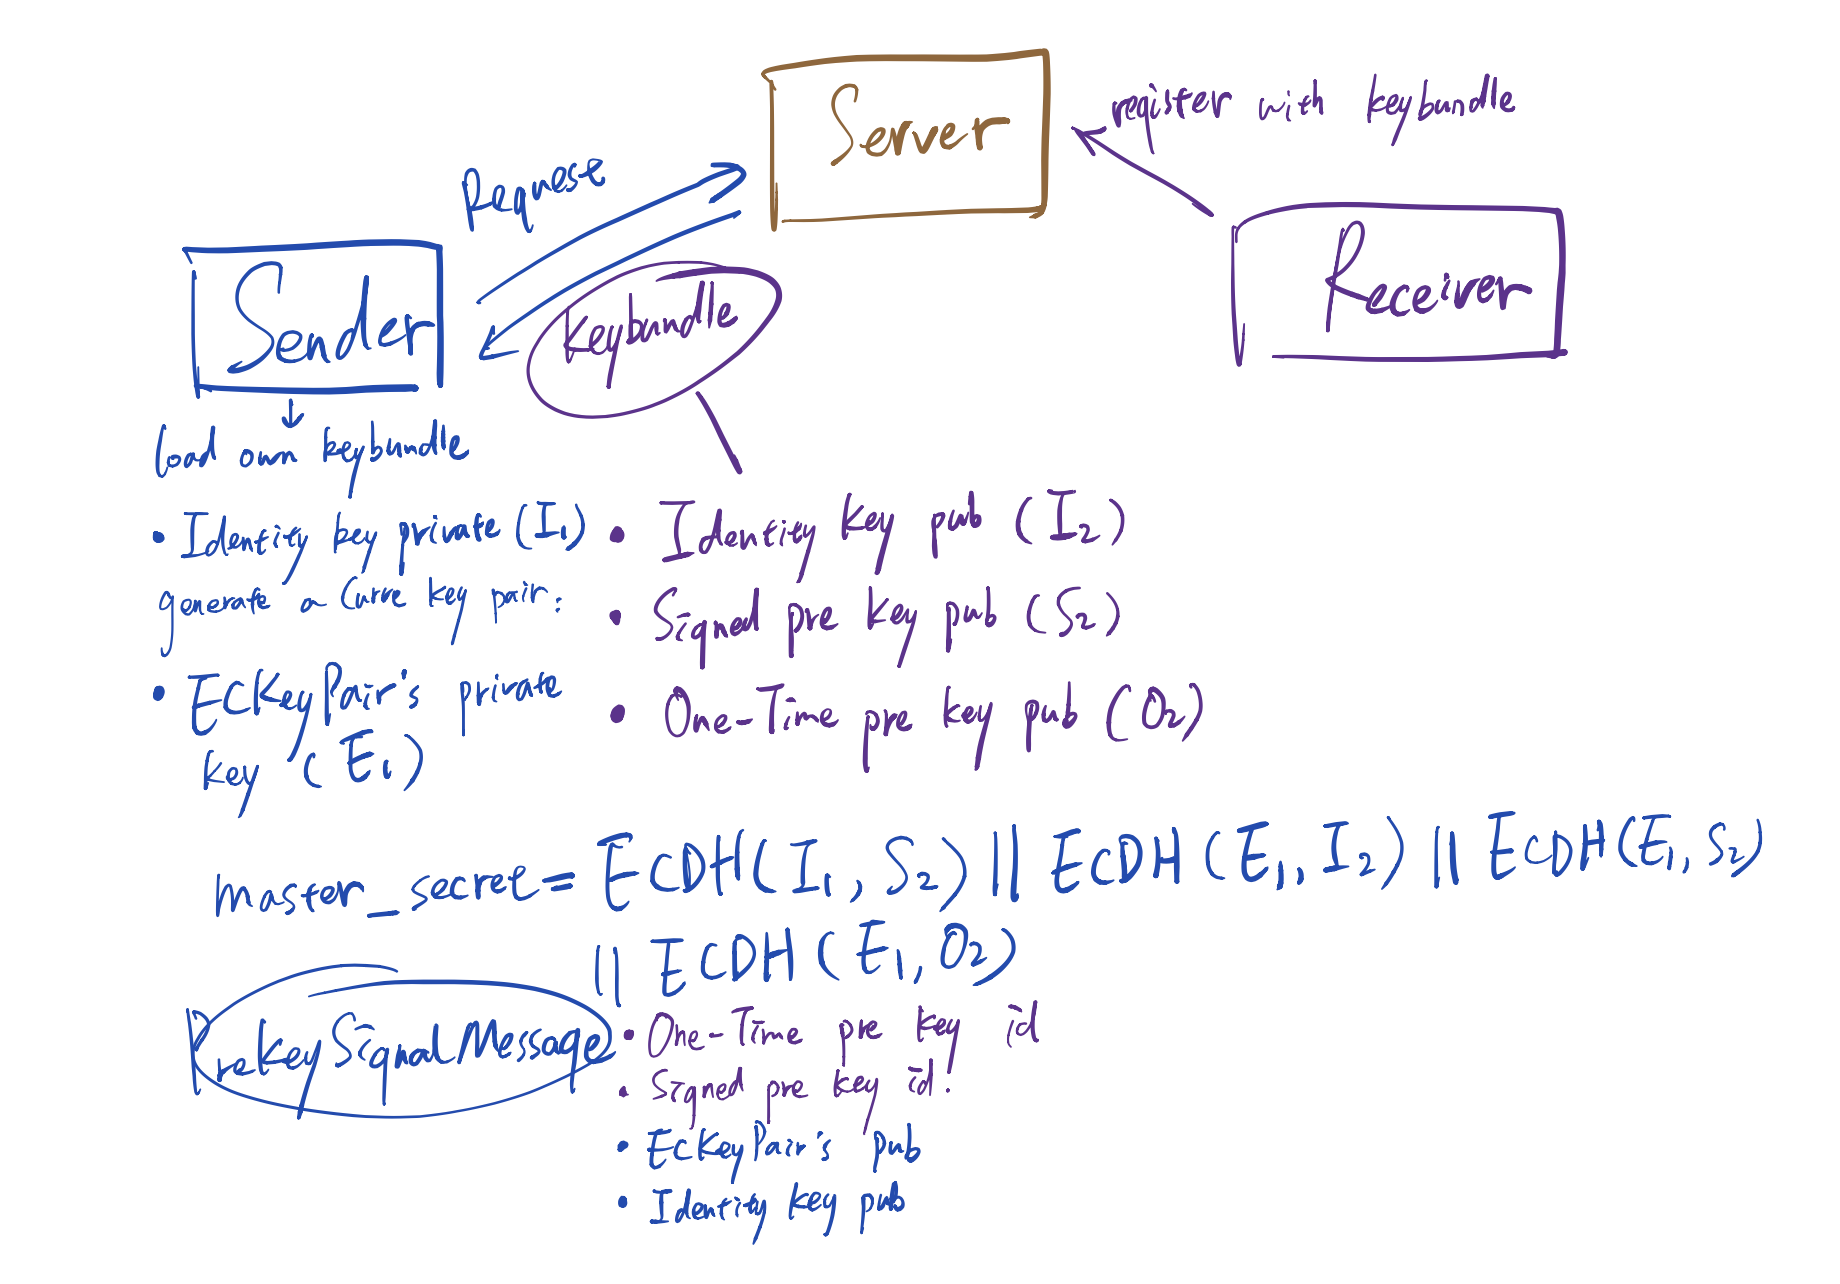
\includegraphics[scale=.5]{../3-Background/resources/X3DH.png}\\
Figure 3.1: \textit{Sender uses Extended Triple Diffie-Hellman Algorithm to initialize the pairwise chat}
\end{center}

Once the master secret is calculated, the sender needs to send his public identity key, the generated public ephemeral key and the receiver's pre keys identifier with the initial message to the receiver.

As mentioned before, the master secret obtained from X3DH is used as the first root key in root chain. Then sender needs to do the first ratchet step in Double Ratchet. The Double Ratchet is formed by DH ratchet and symmetric ratchet. The symmetric ratchet's first chain key is the output of DH ratchet, so sender needs to do the stepping in DH ratchet first. To provide the break-in recovery feature which also means future security, the DH ratchet needs an encrypted input as "salt" in the KDF algorithm. The sufficient entropy of input make the output of KDF appears random which can be used safety as the first chain key in sending or receiving chain.

The input of DH ratchet needs to have enough entropy while it also needs the confidentiality and consistency. So asymmetric encryption is a good solution to solve it. In every messaging package's header, there is a public rathcet key which is used by users to calculate the secret output via DH algorithm. In the initializing situation, receiver's public signed pre key is used as public ratchet key. The sender needs to generate a pair of ratchet keys in the meanwhile and uses the private key of it with the receiver's public signed pre key to do the DH algorithm. The output of it that provides sufficient entropy is used as the input of KDF in DH ratchet's root chain. When sending the message, the sender will send the public key of generated ratchet key pair in message header to make sure the receiver can calculate the same input of KDF in DH ratchet.

After doing the stepping in DH ratchet, root chain generated a new root chain key and a reliable output. The output is used as the first chain key in the second symmetric ratchet which means the first chain key of sending chain or receiving chain. Because the DH ratchet has already added sufficient entropy, so the output of it which is used as the input of symmetric ratchet is reliable that there is no need to add other entropy in symmetric ratchet. So the inputs of symmetric ratchet can be a constant which are usually 0x01 and 0x02. To get the message cipher key, the symmetric ratchet needs to do another stepping by using the KDF in sending chain. One stepping gets a message key which can be used to encrypt the message and once the encryption is completed, the used message key will be deleted immediately to provide the forward security. If the sender wants to send other messages in the same round, the only thing needs to do is doing the corresponding stepping in sending chain to get the right message keys. The figure 3.2 presents the whole process in detail.

\begin{center}
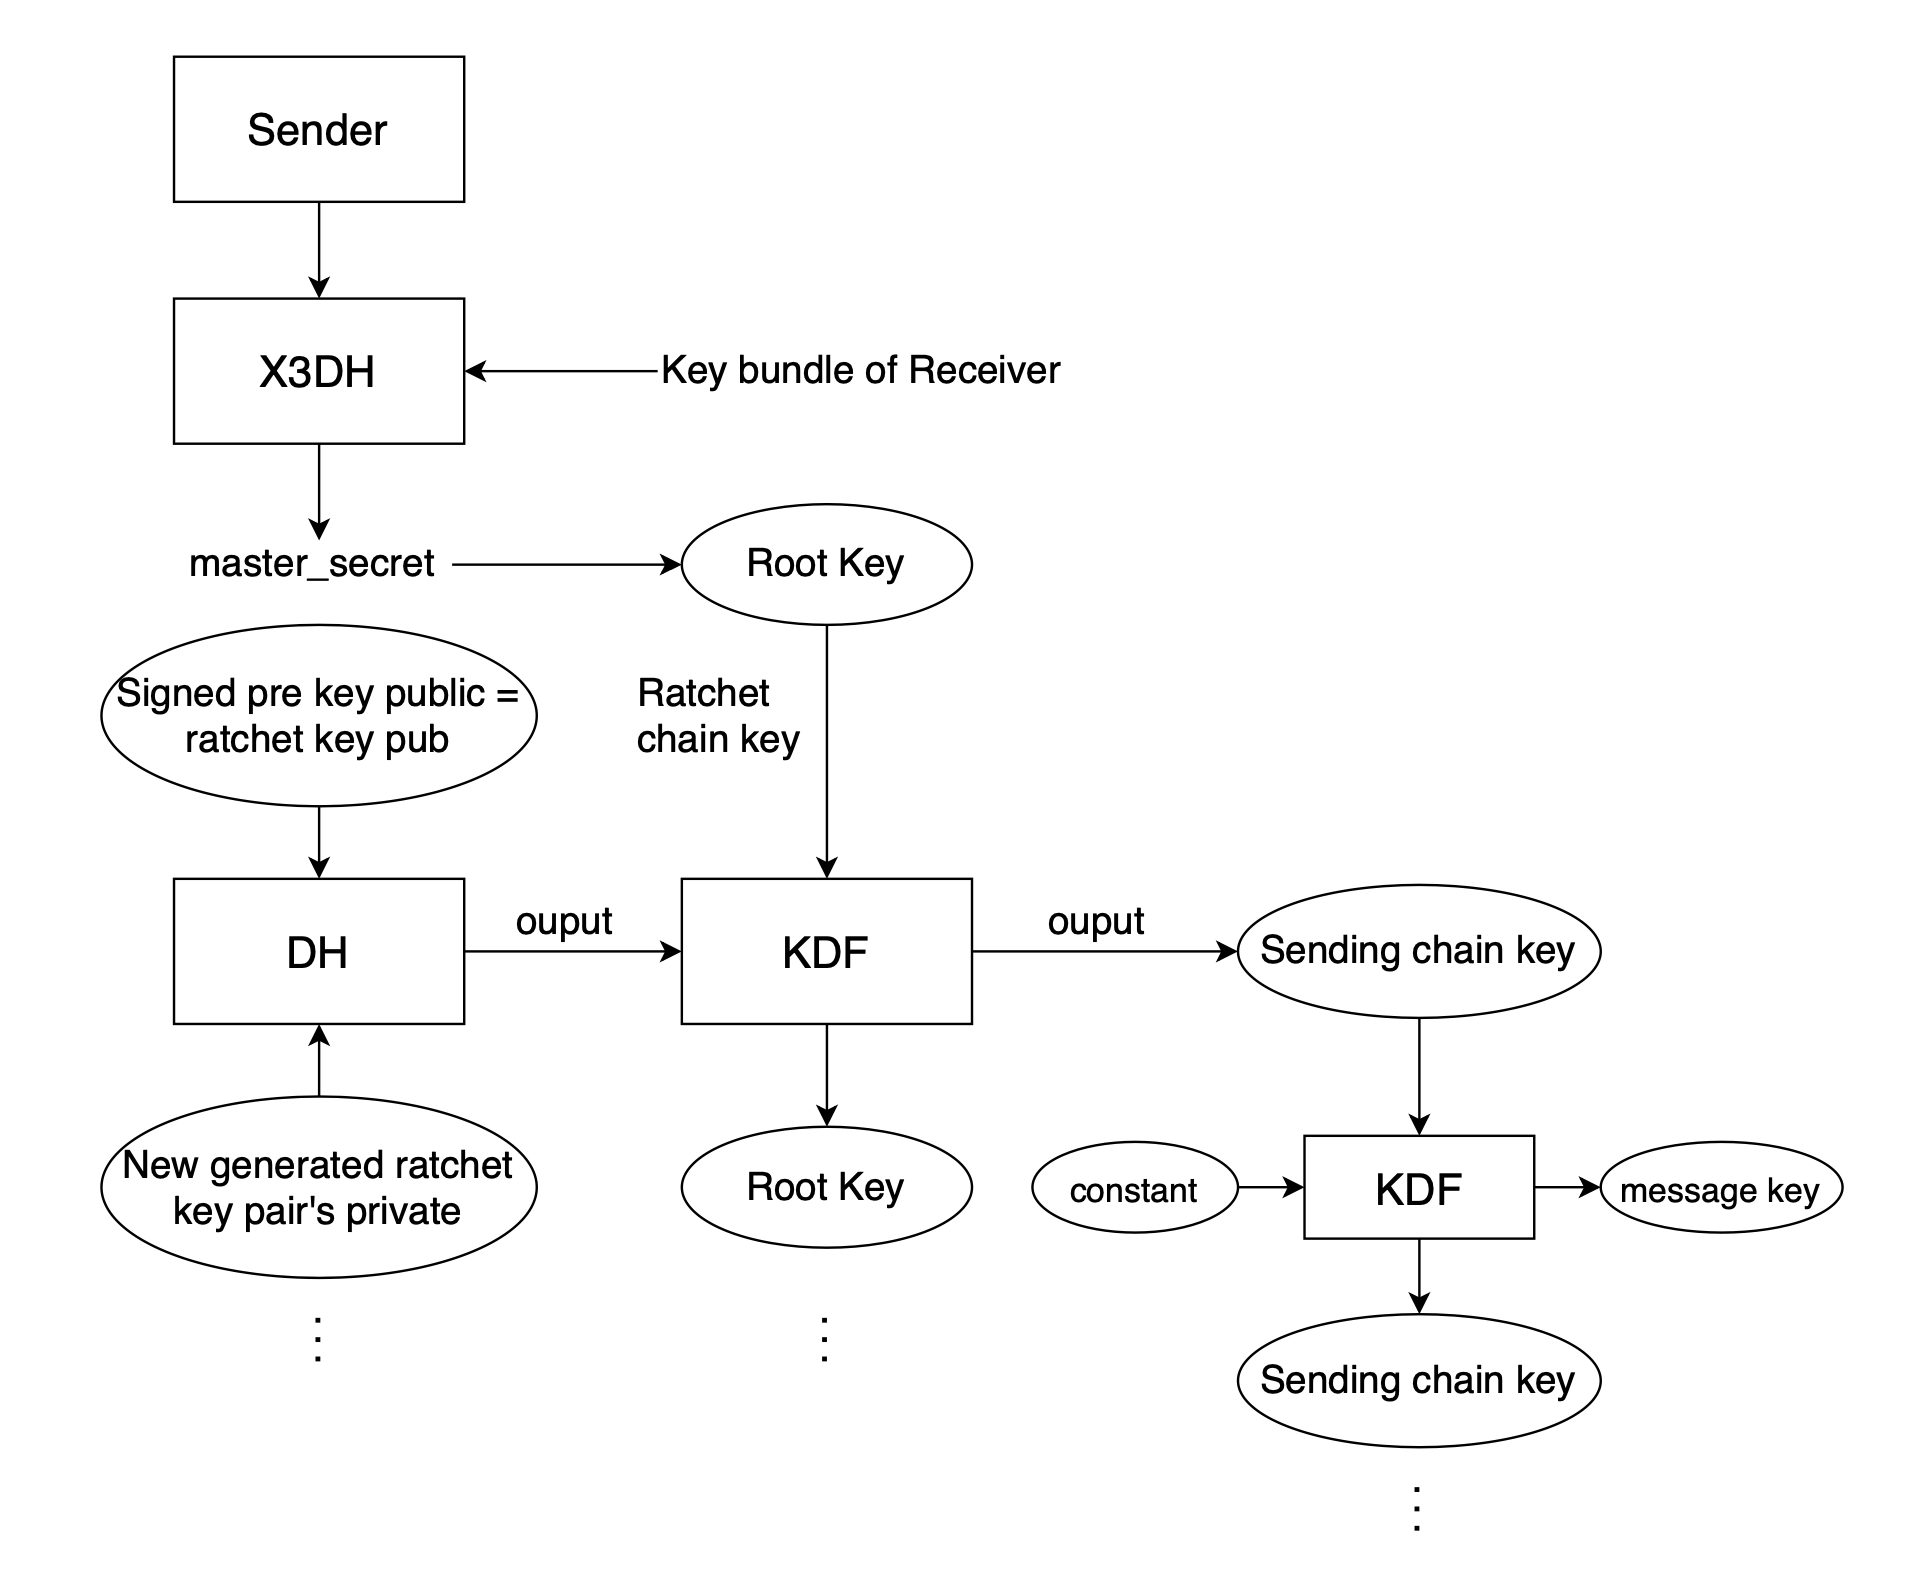
\includegraphics[scale=.5]{../3-Background/resources/DH-init.png}\\
Figure 3.2: \textit{Sender uses the Double Ratchet to encrypt the messages in the initializing situation}
\end{center}

\item Receiving Situation

In the situation that the receiver receives the encrypted messages from sender and wants to decrypt them, if the messages include the X3DH parameters, the receiver needs to calculate the root key first, or the receiver extracts the public ratchet key from message header for further decryption.

Once the public ratchet key is extracted, the receiver needs to judge it with the ratchet states first: if the public ratchet key has the corresponding receiving chain. In the situation that there is not receiving chain corresponds to the received public ratchet key, the receiver uses the old private ratchet key with the received public ratchet key to calculate an output via DH algorithm. Then the receiver uses the output as the input of KDF in DH ratchet's root chain to do a stepping. The output of DH ratchet's KDF will be used as the first chain key in symmetric ratchet's receiving chain as mentioned in initializing situation. Later, the receiver will do the right stepping in receiving chain to obtain the right message key which can be used to decrypt the received messages. Also, for the forward security, once the message key decrypted the messages, it will be deleted immediately. In the other situation that there is a corresponding receiving chain to the received public ratchet key, the receiver gets the right receiving chain and does the proper stepping in symmetric ratchet's receiving chain to get the correct message key.

The Signal Protocol is also designed to handle the out of order messages that may be caused by network delay. If the receiver receives the latter message before the former message, when the symmetric ratchet is doing the corresponding stepping, it will store the generated but never used message key with associated count. Once the former message arrives, the receiver will get the correct message key from stores to decrypt it. The figure 3.3 presents the Double Ratchet's work process in receiving situation.

\begin{center}
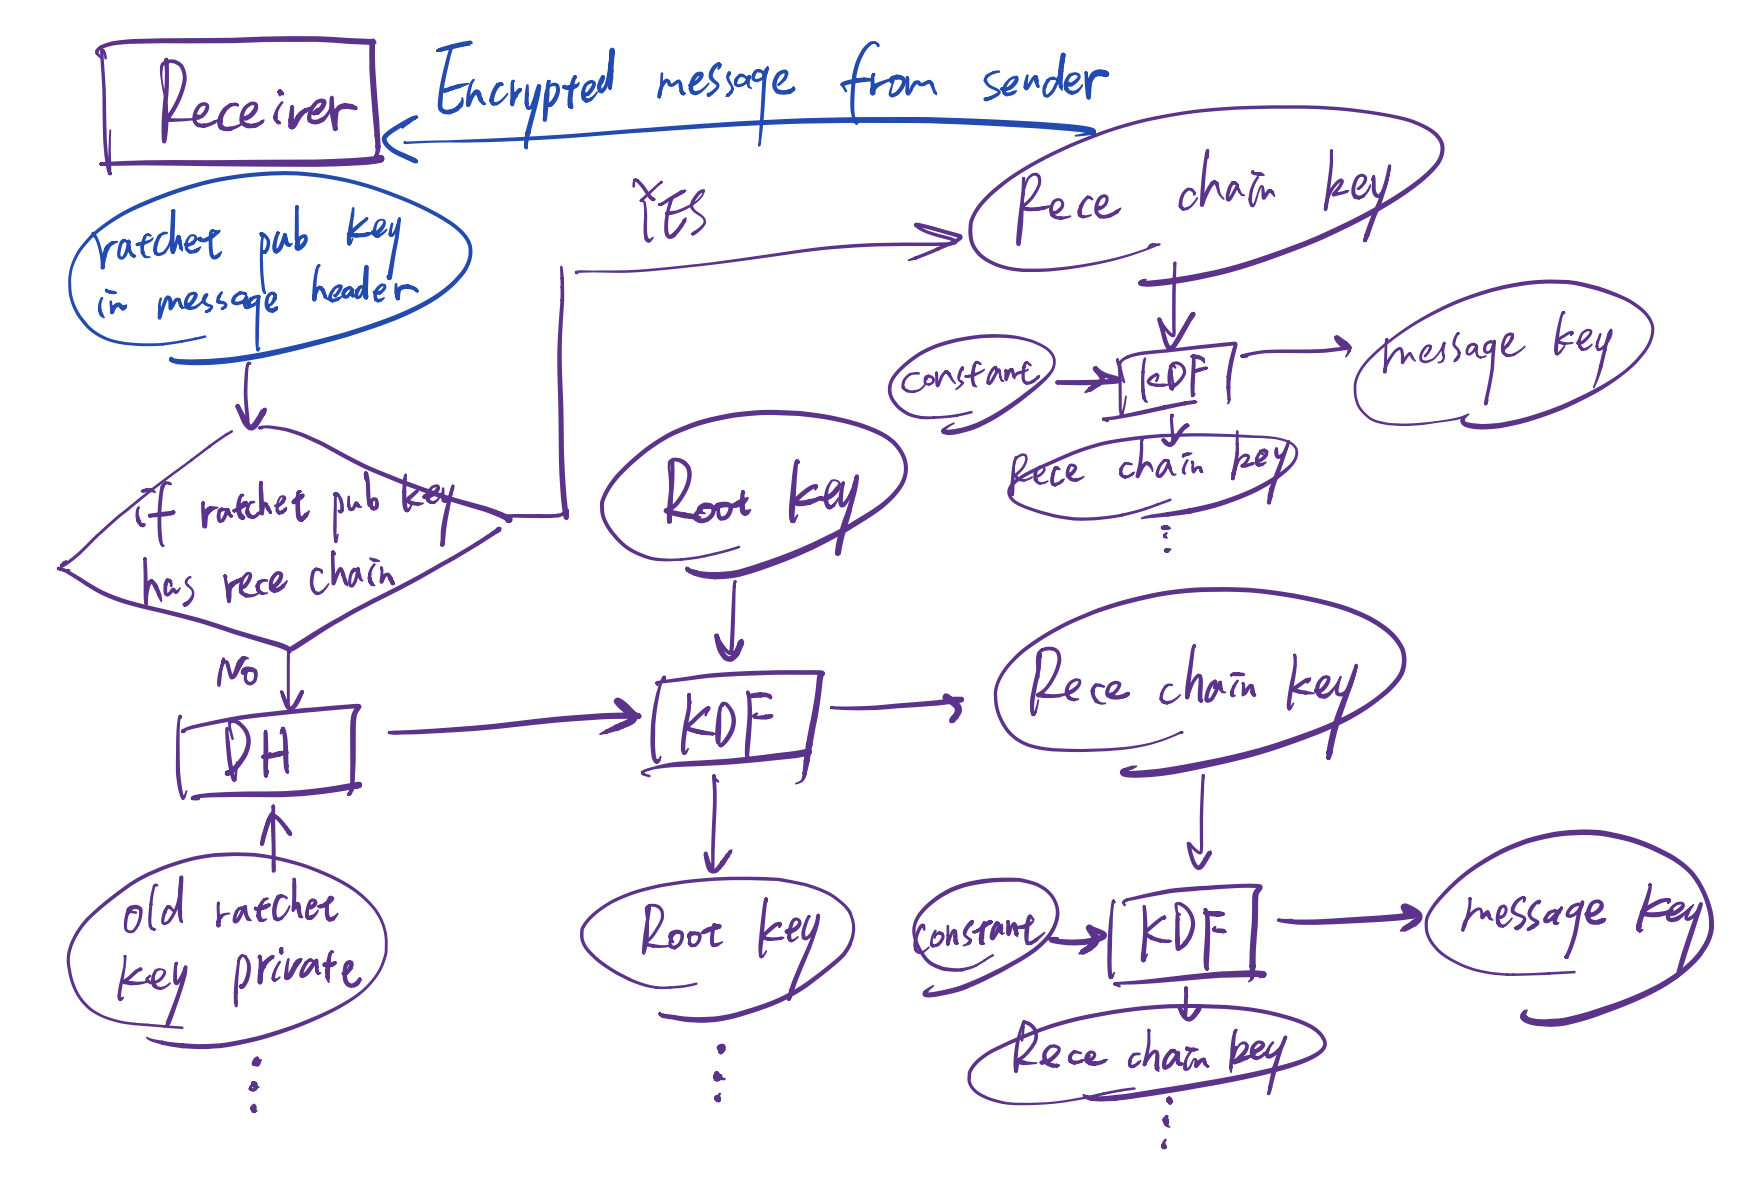
\includegraphics[scale=.5]{../3-Background/resources/DH-rece.png}\\
Figure 3.3: \textit{Receiver uses Double Ratchet to decrypt the messages}
\end{center}

\item Sending Situation

In the situation one party wants to send an encrypted message to others, it's always necessary to generate a new ratchet key pair. The user will extract the public ratchet key in latest message header first, and uses it with the private key of new generated ratchet key pair to calculate the output of DH algorithm. Then the output will be used as the input of the KDF in DH ratchet's root chain and the later steps are almost the same as mentioned in other situations before. Once the message is encrypted and prepared to be sent, the sender needs to add the public key of generated ratchet key pair in message header to make sure the receiver can do the same ratchet stepping. The figure 3.4 presents this process in detail.

\begin{center}
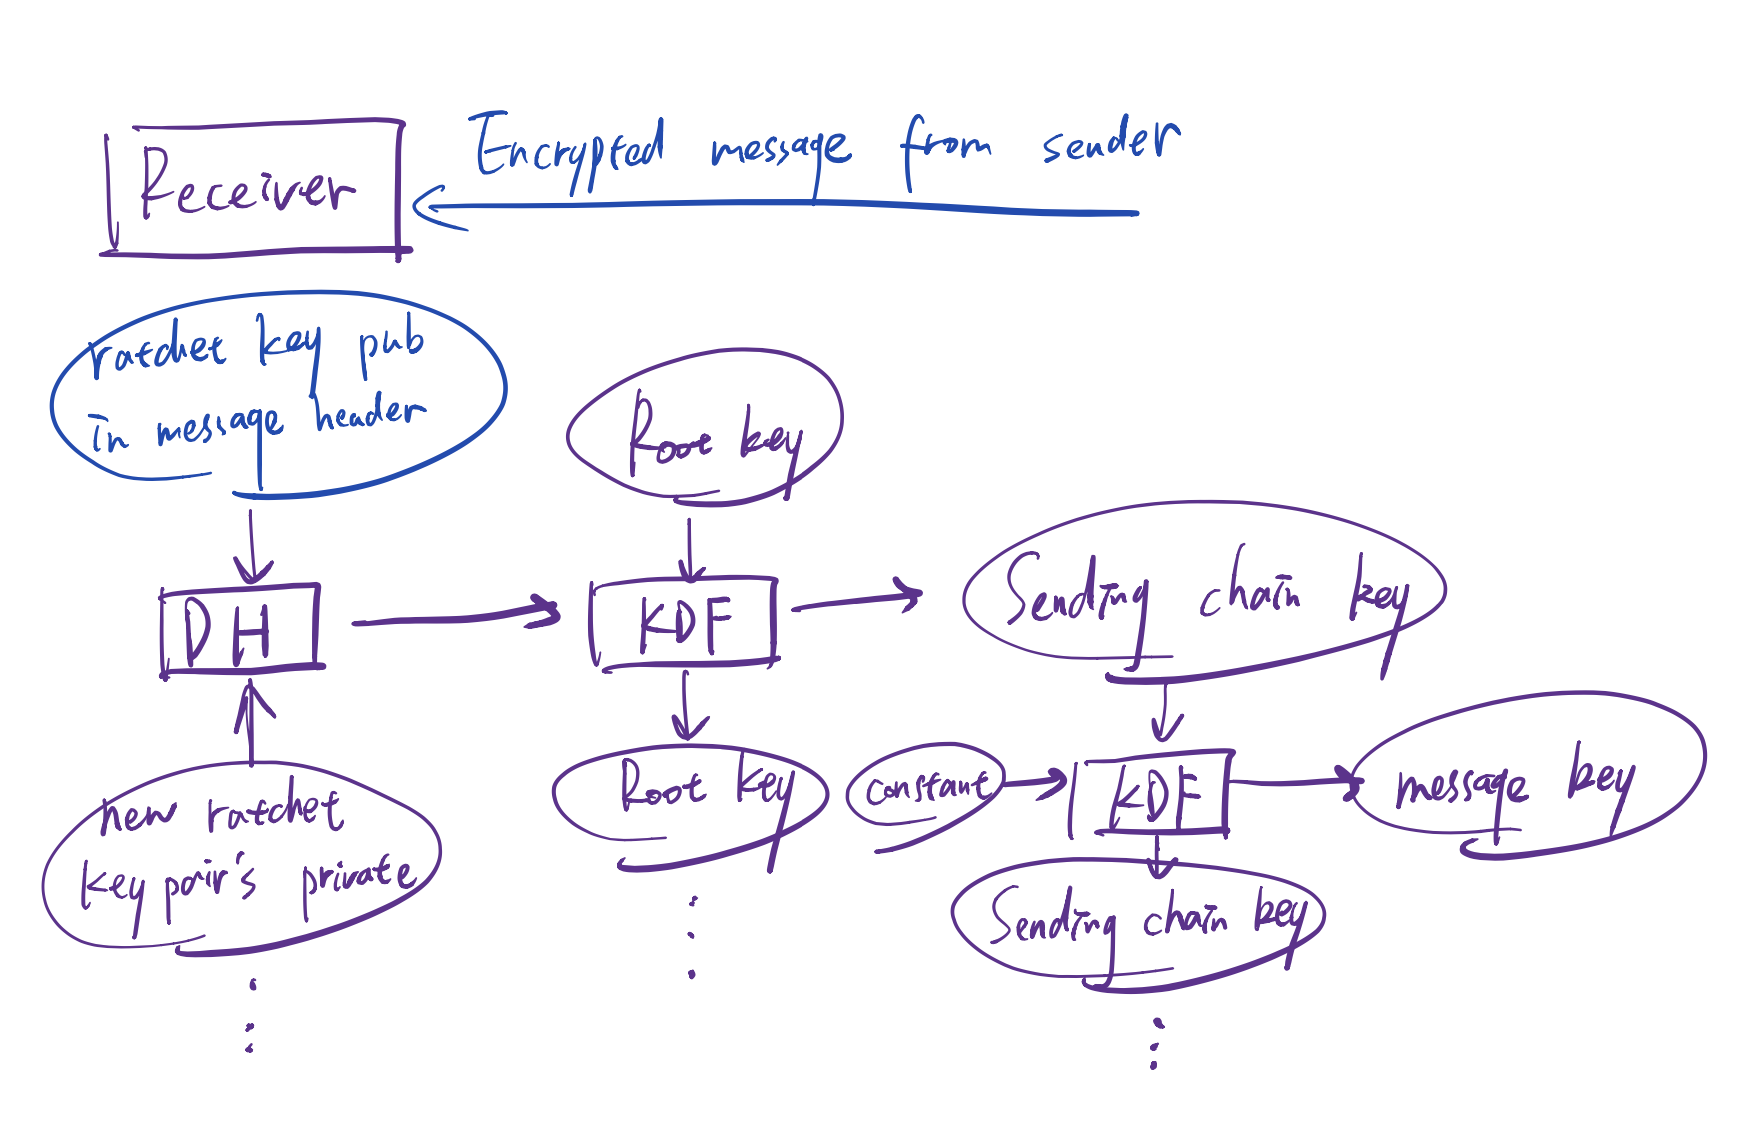
\includegraphics[scale=.5]{../3-Background/resources/DH-send.png}\\
Figure 3.4: \textit{User uses Double Ratchet to send the messages}
\end{center}

\end{enumerate}

\subsubsection{Related Work}
The Signal Protocol is a certain reliable protocol nowadays, there are several applications related to it in our life.

WhatsApp upgrades its application based on Signal Protocol in February 2017 to secure its content. Signal Protocol also has a same name chat application called Signal, which has been used by a lot of people since 2013.

 This project also borrows some strategies from WhatsApp to handle different problems in different situations, like group chat and pairwise chat's fingerprint verification function. However, since this project is developed from an existing chat system, the defect is the communication between the server and the client is special, each side has their own way to handle different type of packages. So the client cannot communicate with other Signal Compatible Server which is a regret. But the idea of Signal Protocol has been implemented in this project, it really improves the security of users' communications.

\clearpage

\end{document}